\documentclass[runningheads]{llncs}
\usepackage{graphicx}
\pagestyle{plain}

\begin{document}
\title{Similarity Resonance for Improving Process Model Matching Accuracy}
\subtitle{Seminar - Selected Topics in Process Mining}
\author{Mukander Kumar}
\institute{Chair of Process and Data Science\\
RWTH Aachen University\\
Germany\\
\email{mukander.kumar@rwth-aachen.de}}

\maketitle     
\begin{abstract}
The procedure of comparing and matching process models is a very robust tool which is now in use for many applications. However, using this tool is not always simple. Developing a similarity model between process activities is one of the prerequisites for comparing and matching process model. To achieve this, this paper uses contextual similarity technique as opposed to existing solutions which only use label-based similarity techniques. The paper describes contextual similarity as a method of gauging the similarity of context between two activities, It is accomplished through the use of similarity resonance, a recurrent algorithm for determining global contextual similarity among process activities. Basically, the pairwise similarity among all process activities is calculated and modified iteratively based on the similarity among their neighbours until the similarity scores are stabilised and propagated to the entire graph \cite{ref2}.
\end{abstract}
%
\section{Introduction}
The significance of process model matching has increased with the advent and rise of a huge number of process model repositories which need to be handled properly\cite{ref3}. A similarity measure allows the activities of two or more process models to be mapped properly. The task of matching two process models is divided into two phases: (i) calculating the pairwise similarity among activity labels, and (ii) obtaining the mapping among activities, taking into account the structural factors and behaviors, and optimizing the maximization of certain objective function.\newline 

The consistency of the activity similarity determines the accuracy of the mapping, so if two activities are marked as similar in the first step, there is a high chance that the activity will be mapped similarly in the second step\cite{ref6}.Therefore, improving the similarity of the tasks will increase the matching precision of the process model. The context of an activity is represented by its neighbourhood. Then, if the neighbourhoods of two activities are comparable, they are considered similar. This leads to an iterative approach in which similarity scores between activities are assigned based on their neighbors’ similarity\cite{ref8}, and the obtained similarity scores are promulgated to neighboring activities until convergence. This paper solves the problem of using a structured approach to calculate effective measures of similarity between activities. In general, activity similarity is measured by comparing the syntactic (e.g., Levenshtein distance) and semantic (e.g., WordNet) similarity of their labels. However, in this approach, crucial information about the context in which tasks are carried out is ignored. The similarity computation's accuracy suffers as a result. To address these constraints, the paper devised a mechanism for automatically calculating the total contextual similarity of activities as the background data provided by the activities will support the calculation of an even more accurate similarity. %
\section{Related Work}
To address the challenge of process model matching, many articles are been published:
\begin{itemize}

    \item[$\bullet$] The paper \textit{"Spectral methods for global alignment of multiple protein networks" }and\textit{"A versatile graph matching algorithm and its application to schema matching"} introduces the concept of recursively calculating nodes and similarity scores based on neighborhood and has already been analyzed in a variety of areas.\newline
    
    \item[$\bullet$]The paper \textit{"The Page Rank citation ranking: bringing order to the web"} handles the problem in a way similar to Google’s PageRank algorithm for prioritizing nodes on graphs.\newline
    
    \item[$\bullet$] \textit{"Using information content to evaluate semantic similarity in a taxonomy"} provides semantic similarity metrics for determining the level of semantic similarity between activity pairings.\newline
    
    \item[$\bullet$] \textit{"Discovering context-aware models for predicting business process performances"} and \textit{"Discovering context-aware models for predicting business process performances"} use a clustering methodology where the traces are separated into separate groups depending on their context characteristics, and a prediction model for each cluster is developed. The prediction then identifies the cluster that best fits the partial trace of the process instance that was supplied.\newline
    
     \item[$\bullet$] The paper \textit{ "A case-based reasoning framework for workflow model management"} has workflow examples from a repository of process models, and a novel framework to facilitate workflow modeling and design.\newline
     
       \item[$\bullet$] The paper \textit{The paper "How to Make Process Model Matching Work Better? an analysis of current similarity measures" }attempts to answer this question by conducting two separate analyses reviewing existing process model matching techniques and analyzing the Process Model Matching correspondences.\newline
       
         \item[$\bullet$] The paper \textit{"Efficient process conformance checking on the basis of uncertain event-to-activity mappings"} presents a probabilistic conformance-checking approach that can cope with uncertain mappings by eliminating the requirement to choose a single mapping by taking into consideration the whole spectrum of potential mappings.
\end{itemize}

\section{Preliminary Definitions}
Some important definitions to understand the approach of the paper are as follows: 
\begin{itemize}
    \item[$\bullet$] \textbf{Event:} An event consists of the process activity \textit{a}, its case id \textit{c}, its timestamp \textit{t} and a list of all additional attributes as \textit{di.......dm}. This is stored in the form of a tuple such that \textit{e = (a, c, t, di……dm)}.\newline
    
     \item[$\bullet$] \textbf{Process Model:}  A process model is a graphical depiction of a particular process. The modeling might be based on a variety of notations and standards, including BPMN 2.0.\newline
    
     \item[$\bullet$] \textbf{Preset/Postset:} The preset and postset of the activity pair are defined as the backward and forward linked activity pairs in a process respectively. \newline
    
    \item[$\bullet$] \textbf{K-nearest-neighbor:} It is a data classification algorithm that looks at the data points surrounding it to decide which group a data point belongs to. The algorithm examines one point on a grid to determine whether it belongs to group A or B by examining the state of the points nearby. \newline
    
    \item[$\bullet$] \textbf{Shortest activity path:} In a process model, it is defined as the shortest distance between various activities. Generally, the similarity of activities is determined by calculating the syntactic distance, such as the Levenshtein distance.\newline
    
    \item[$\bullet$] \textbf{EigenValue:} Eigenvalues are a subset of scalars correlated with a linear system of equations (i.e., a matrix equation), and they are sometimes referred to as characteristic roots, characteristic values, suitable values, or latent roots.\newline
    
    \item[$\bullet$] \textbf{Trace, Partial Trace:} A trace is a finite sequence of events and a partial trace represents an instance which has not been completed yet.\newline
     \item[$\bullet$] \textbf{Similarity matching:} Based on the label metrics, similarity matching attempts to detect similar behaviors.If two entities are similar in some way they share other characteristics as well.\newline
\end{itemize}


\section{Structure}
The term paper has been divided into 7 sections:

\begin{itemize}
     \item[$\bullet$] \textbf{Section I} demonstrates how process model matching is a recurring theme and how it is directly related to accuracy. It provides a brief overview of the limitations of standard process model matching approaches, as well as a strategy to address the mentioned limitations. \newline

    \item [$\bullet$] \textbf Section II represents how different approaches have been used in the hope of addressing the challenge of process model matching and briefly reviews previous work \newline
    
    \item [$\bullet$]  \textbf Section III provides the basic definitions and notations needed to comprehend the work presented in this term paper.\newline
    
    \item [$\bullet$]  \textbf Section IV explains the problem statement and provides a summary of the proposed solution.\newline
     
    \item [$\bullet$]  \textbf{Section V} outlines a three-step method for calculating pairwise similarity resonance score among activities.\newline
    
   \item [$\bullet$]  \textbf Section VI explains the results obtained by running experiments on various datasets.\newline
    
    \item [$\bullet$]  \textbf Section VII discusses the overall conclusion of the paper as well as future work.
\end{itemize}

\section{Approach}
We analyse an example in this section to explain our method. Consider the two birth registration process models (sub-processes) as shown in Figure 1 of the paper. Assuming that instances marked with the same numbers should be matched according to some ideal baseline, we calculate the pairwise similarity of the process activities. The graph edit distance is used to remove the structural dissimilarity of the activities. Column SimL in Table 1 of the paper displays a sample of the similarity scores obtained using label-based similarity. We obtain the matching set M= 0.3 through the use of a matching algorithm, e.g. the graph edit distance with a threshold of t= 0.32. Table 1 pairs have a higher than 0.3 similarity value, except for the pair (Return documents 2, Return documents). Because of their dissimilarity, the pairs labelled 5 and 6 on the table will not be recognized by a matching algorithm\cite{ref10}.\newline 

As we observe the environment in which these tasks are carried out, we can confirm that both activities are carried out after verifying the newborn's identity and before the procedure ends, with refusal of continuation and cancellation of birth notification occurring concurrently. Following a review of the personal records, "Run through data" and "Search GBA" are simultaneously carried out. Return documents and Return documents 2 are also performed in totally different contexts, as shown.\newline 

Using the above illustration, we recommend the similarity calculation between two activities by comparing the similarity between their k-nearest neighbouring activities. The recently computed similarity will be propagated throughout, growing the similarity of the neighbours' as a result. This forms an iterative method in which similarity scores are calculated recursively and spread to neighbours until convergence\cite{ref18} .The method can be devolved into three major steps: 
\newline 
(1) Derive each activity’s k-nearest neighbours in the input process models.
(2) Derive the k-resonance graph.
(3) Determine the pairwise similarity resonance scores by solving an eigenvalue problem.\newline 


In Table 1 of the paper, the column SimR displays the similarity resonance scores computed using the paper's similarity resonance technique. Two hypotheses are presented based on the findings. Firstly, the SimL = 0.14 and SimL = 0.13 similarity scores for matches 5 and 6 went up to SimR = 0.29 and SimR = 0.31, respectively. The algorithm can thus recognize these matches with a t = 0.3 threshold.  On the other hand, the similarity score of (Cancel birth notification, receive notification of birth) went down from SimL = 0.35 to SimR = 0.07. The matching algorithm can now exclude this activity pair. Furthermore, the similarity score of (Return documents 2, Return documents) has gone down to SimR = 0.21 from SimL = 1.0. This activity pair was thus excluded using a matching algorithm that didn’t consider the structure of the process model. Second, the similarity scores of matches 1, 2, 3, and 7 decreased and were of little consequence as some dissimilar neighbours which surrounded the activities were held responsible for the decrease\cite{ref12}.However, with the highest similarity score, these pairs remained the strongest. We'll see how to monitor the amount of similarity that a neighbour will contribute in the next segment.

\subsection{K-Nearest Neighbour}
The basic function of the  K-nearest neighbour is to get contextual similarity which is main goal in our algorithm. As we know that not only labels but also the context is more important process model matching accuracy \cite{ref17}.The intuition of the algorithm which is proposed (i.e. similarity resonance) aims to assess that not only the label metrics, but neighboring activities, also contribute indirectly to the similarity in the graph, so we assume that the k-nearest neighbours have a direct influence on the accuracy. When calculating the k-nearest neighbour, we look at the preset and postset, the preset and postset for the running example are defined in figure 1.
\begin{figure}
    \centering
    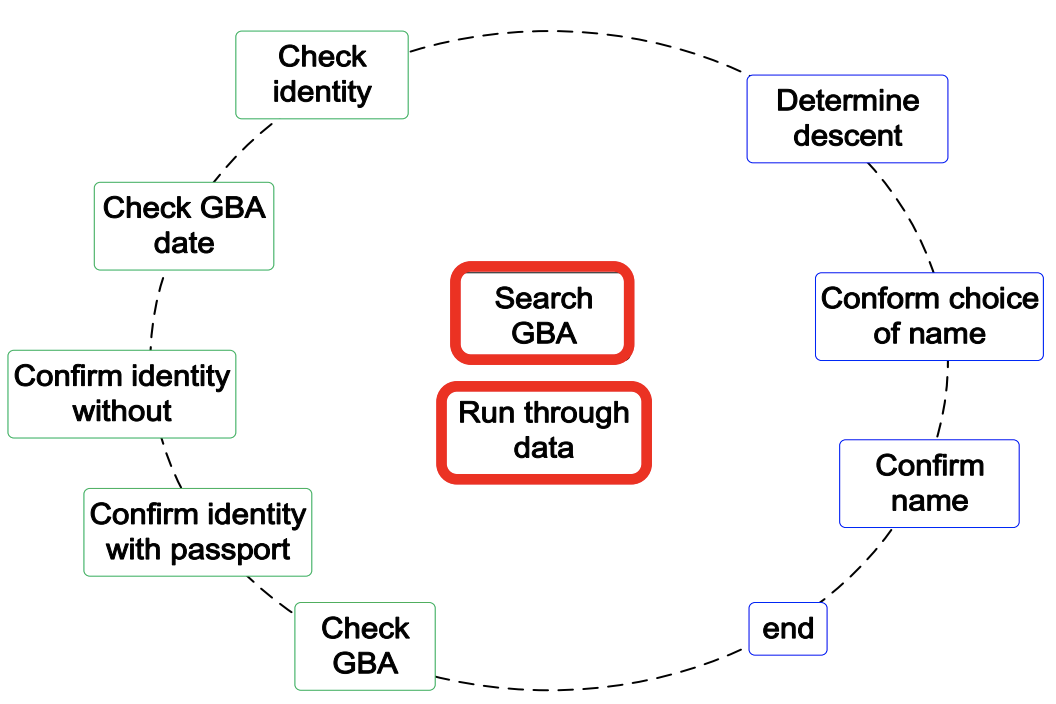
\includegraphics[width = \textwidth]{Figures/Fig_1.PNG}
    \caption{Nearest Neighbors for  '"Search GBA" and "Run Through data"}
    \label{fig:1}
\end{figure}


\subsection{K Resonance Graph}The second stage is to specify how the similarity between the activity pairs and their neighbors will be transmitted. To do this, we create a weighted directed graph, known as a k-resonance graph. The graph's nodes represent all conceivable activity pairings in Figure 1. An edge connecting two nodes indicates that the similarity of the source node to the destination node. An edge exists between a source node and a target node if both activities of the source node's activity pair correspond to the k -preset or k -postset of the target node's activity pair.The propagation coefficient, which is the amount of similarity transmitted from the source to the destination node, is shown by the edge weight\cite{ref11}.\newline

The purpose of the edge lies in the fact that the correct matches will get more weight than the less likely matches. A node's similarity to a specific neighbor is defined as the proportion of the neighbors' factors divided by the total of all the neighbors. We do so by giving a higher weighing coefficient to the correct matches so the resonance score can get a higher SimR score, because we want the correct matches to be on the final resulting graph, which will improve the accuracy. By giving less weighing coefficient to less likely matches will lead to downside in the SimR score, we will then eliminate these activities that will also lead to an increase in accuracy.

\begin{figure}
    \centering
    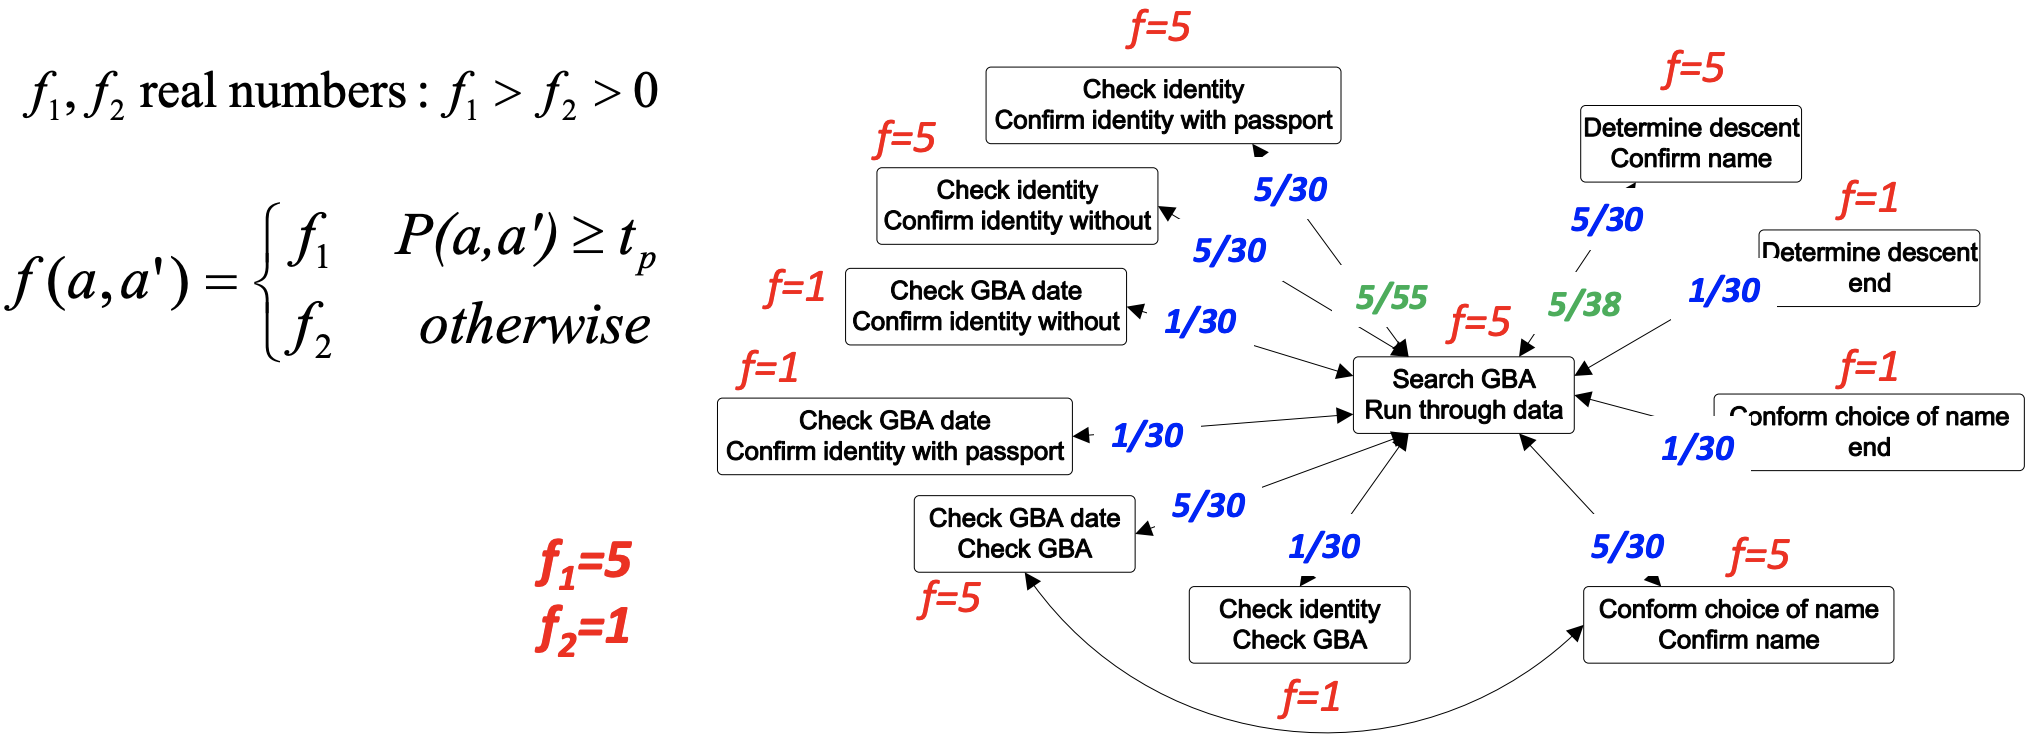
\includegraphics[width = \textwidth]{Figures/Fig_2.PNG}
    \caption{The 2-resonance graph that leads to the process model mentioned in Figure 1}
    \label{fig:2}
\end{figure}
\subsection{Mathematical Expression}
Following the formation of a transition system, each state is annotated with the Naive Bayes classifier and each event with the Eigen value, which is trained on the event log including previous data in BPMN 2.0. The classifier's aim is to find the likely similar match , whereas SVR is used to estimate the similarity among nearest neighbor. Equation will give the likely similar match obtained by the present annotated transition system.\cite{ref18}
\begin{figure}
    \centering
    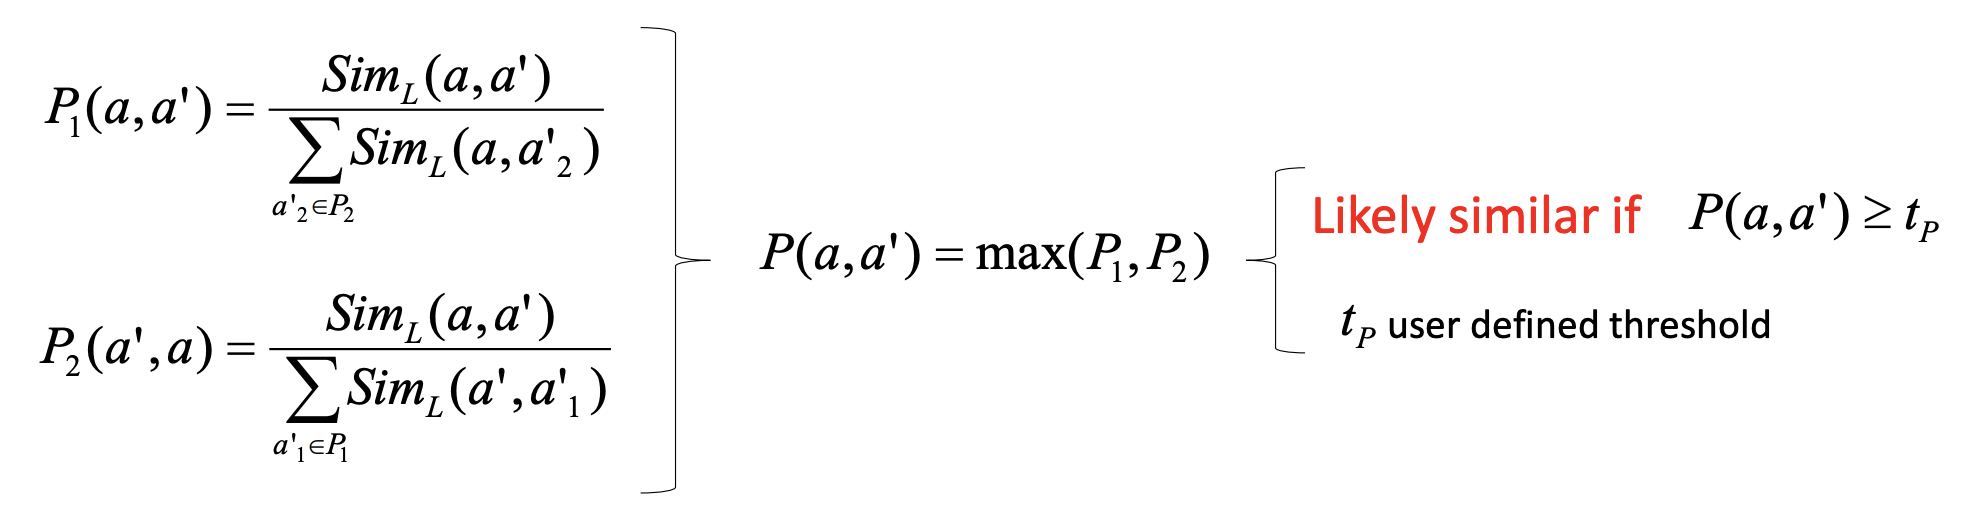
\includegraphics[width = \textwidth]{Figures/Fig_3.PNG}
    \caption{Mathematical Expression \cite{ref22}}
    \label{fig:3}
\end{figure}
\subsection{Similarty Resonance}
The similarity resonance scores are derived recursively based on the similarity of the neighbors in the k-resonance network. The algorithm ends when a fixpoint is reached, i.e. when all similarity values are stable. The calculation is divided into two steps: I initialization and (ii) iteration. SimL is used to generate initial similarity scores during the initialization process. Throughout the iteration the scores are recursively updated depending on the similarities of neighbors.

\section{Tools and Parameters}
The tools used for the implementation are \textit{Prom} and \textit{BPMN} framework. The transition system and has been built as a prom plugin and BPMN framework has been used for the implementation on various datasets.The implementation is very easy and does not involve adjustment of bulk of parameters. For the K-nearest neeighbour you must specify the number of K you wish to choose and the recommended is more than 1. For K-resonance graph you have to assign the fractions to neighbour and non- neighbour. However, real-world data from the Process Model Matching Contest are available also (PMMC).

\section{Comparison}
To make sure that the results provided by this technique are better than the previous ones, the results were compared with the previous standard label similarity technique.  The aim was to compare with several other freely available datasets such as birth registration (petri net) containing 9 process models, 36 process pairs to match, University admission (bpmn) with 9 process models, 36 process pairs to match and Asset management (EPC) with 36 pairs of process models retrieved from SAP.
\newline\newline
The comparison was based on 3 experiments. The first one is accuracy of process matching using standard label similarity vs using resonance similarity. Second, the best findings from PMMC'16 and OAEI'16 were compared and finally impact of changing the alpha and k of the similarity resonance on accuracy. As a similarity measure, the standard label similarity uses the bag-of-words approach in connection with the maximum between Levenshtein distance and Lin metric. In matching algorithms there were graph edit distance with default values and 2 variants of a greedy algorithm (1:n and 1:1 mapping)\cite{ref14}. Before picking the best match, we also tested with the matching algorithms' cutoff levels.(in comparison to the total F-score).As a result the following parameters have been modified: k has been increased from 1 to 3;  By increasing 0.1 in each stage, alpha is increased from 0.1 to 0.9 and the cutoff threshold is changed from 0.1 to 1 by adding 0.05 in each step by changing the weights of the operations (substitution, deletion, and insertion) in the graph edit distance. We utilized weight 1 for each operation since the outcomes were better than using the weights recommended in [3].


\section{Application}
An application could be an online and manual admission procedure for different universities (A and B). The process could be that two different students try to obtain admission offers from two different universities. Assume university A has an online admissions process, while university B has a manual/paper-based admissions process. University A receives online applications and University B receives paper-based applications. After that, both the universities check the documents provided by the applicant. After that, University A invites its applicant to an interview, whereas University B invites its applicant to take an aptitude test.The activities are intended to assess whether or not a candidate is a suitable fit for a university. At the end of the admission process, university A sends a decision letter and university B informs the applicant about their application being successful or not. If we apply the label-based similarity metrics, then the correlation is evident between "Receive online application" and "Receive application form" from both University 1 and University 2 respectively.\newline
\begin{figure}
    \centering
    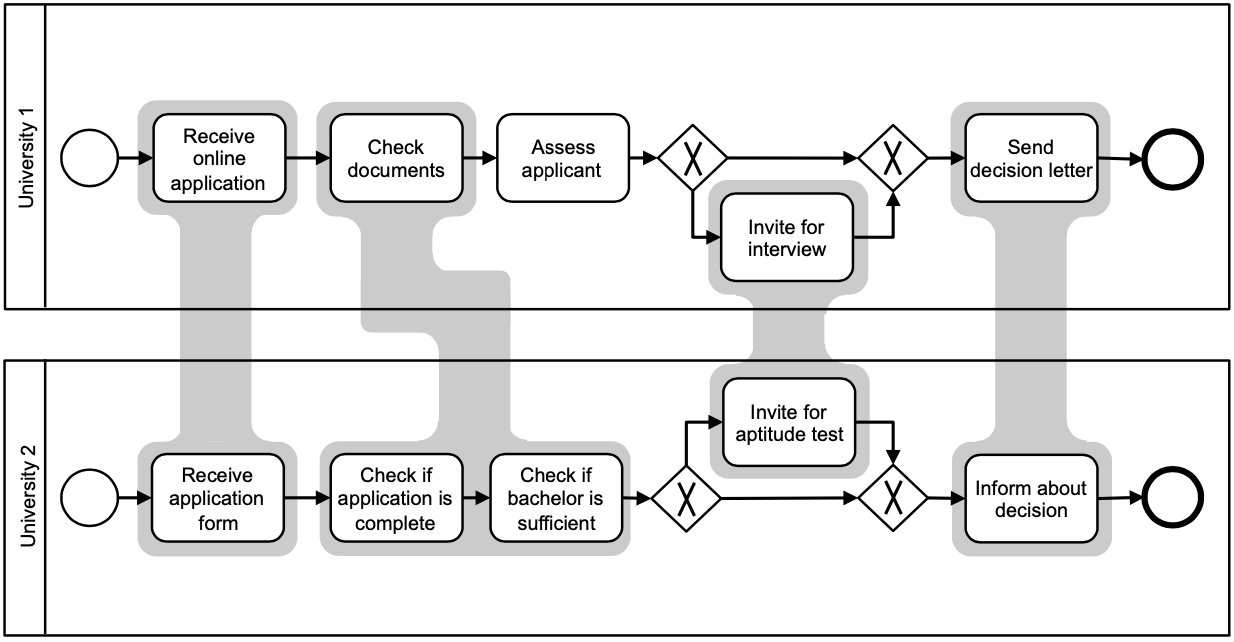
\includegraphics[width = \textwidth]{Figures/Fig_4.PNG}
    \caption{Two University Admission Process models with intended blocks for activity matching.\cite{ref5}}
    \label{fig:4}
\end{figure}
However we can make the argument that this correlation is preferable because it both defines the confirmation of an application document. However, we may argue that the two activities have nothing in common, because the first pertains to an online method and the second to a paper-based setting.Similarly, the connection between "invite for aptitude test" and "invite for interview" may be established because both activities are designed to determine whether or not a candidate is a good fit for a university. An interview, on the other hand, is plainly not the same as an aptitude test, making the correspondence questionable. These examples show how difficult, if not impossible, it may be to get an agreement on a single precise set of correspondences. Adding similarity resonance and matching activities based on context and nearest neighbors will thus address the matching technique problem.\newline

In the first stage, we calculate the K-nearest preset followed by the postset of the activity pairs, because not only neighboring but also other activities have a significant impact on the similarity metric of the two activities. Figures 5 and 6 depict examples of the activities requested for the aptitude test and an interview with the two nearest neighbors.
\begin{figure}
    \centering
    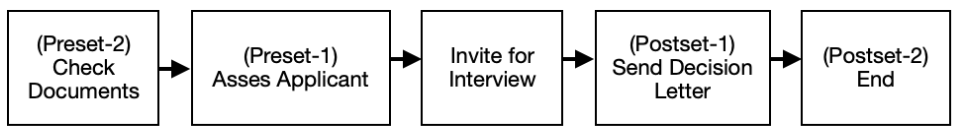
\includegraphics[width = \textwidth]{Figures/Fig_5.PNG}
    \caption{2-Nearest Neighbors of Invite for Interview}
    \label{fig:5}
\end{figure}
The second step is to calculate K-resonance graph, we compute it by propagating the similarity among the activity pairs and their neighbors.
\begin{figure}
    \centering
    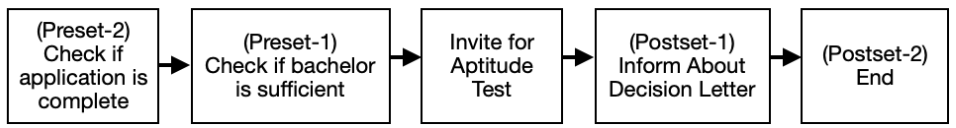
\includegraphics[width = \textwidth]{Figures/Fig_6.PNG}
    \caption{2-Nearest Neighbors of Invite for Aptitude Test}
    \label{fig:6}
\end{figure}
Figure 7 shows a perspective of the resonance graph in connection to the process models given in Figure 4. The graph depicts two activity pairings (Invite for Aptitude Test and Invite for Interview) as well as the nearest preset and postset. For example (Invite for aptitude test and Invite for interview), the two closest presets are (Invite for interview) = assess the applicant and check documents (Invite for aptitude test) = check if the application is complete and check if the bachelor is sufficient. The 2-nearest preset's four potential activity pairings are linked to Invite for interview and Invite for aptitude test and therefore contribute to their similarity, as does the 2-nearest postset. The second stage is to specify how the similarity among the activity pairs and their neighbors will be transmitted. To do this, we create a weighted directed graph, known as a k-resonance graph.\newline

The nodes of the network reflect all possible activity pairings in Uni1 and Uni2. The presence of an edge between two nodes indicates that the source node's similarity to the destination node has been transmitted. An edge exists between a source node and a target node if both activities of the source node's action pair correspond to the target node's k-preset or k-postset. The propagation coefficient, which is the amount of similarity transferred from the source to the destination node, is reflected by the edge weight. The similarity factor for the less likely matches is 1.0, while the similarity factor for the more likely matches is 5.0. A node's degree of similarity to a particular neighbor is computed as the proportion of the neighbor's factor divided by the sum of all the neighbors' factors. The first criteria is self-evident; a big L indicates a high likelihood of a correct match. It should be emphasized that after utilizing similarity resonance, this hypothesis may become incorrect,However, that is our best guess to begin with. The second criteria indicates the level of ambiguity. The two activities might have a high or low similarity value, but the activity pair always has a high factor of similarity. Figure 7 shows a section of the 2-resonance graph matched to the process models shown in Figure 4.\cite{ref3}
\begin{figure}
    \centering
    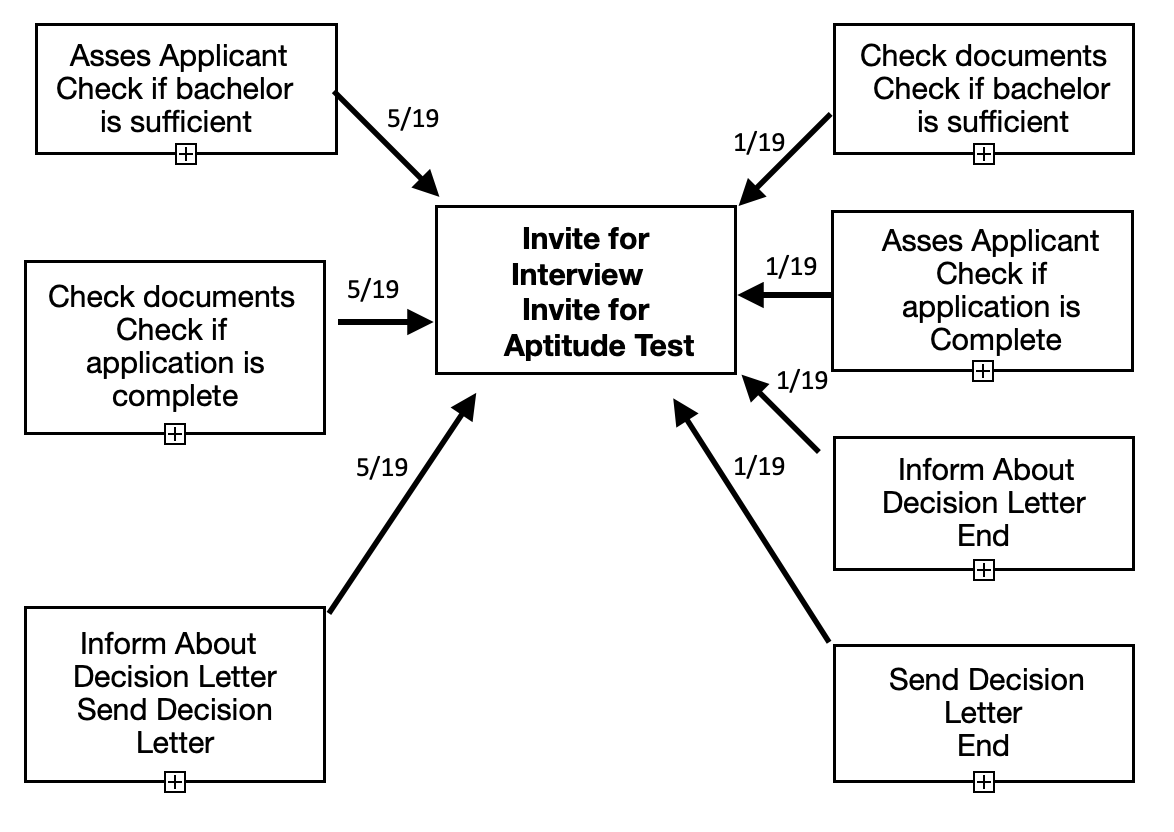
\includegraphics[width = \textwidth]{Figures/Fig_7.PNG}
    \caption{The process activities represented by a two-resonance graph, depicted in Figure 4.}
    \label{fig:7}
\end{figure}

The data shows one activity pair (invitation to an aptitude test and invitation to an interview) and their connections to the two closest presets and postsets. Consider the following scenario: (Invite for aptitude test and Invite for interview), 5/19 is the amount of similarity received from neighbors from (Check whether a bachelor is sufficient, Assess Applicant), (Check papers, Check if the application is full), and (Inform About Decision Letter, Send Decision Letter) 1/19 from (Check documents, Check whether a bachelor's degree is adequate), (Assess Applicant, Check if the application is complete, etc.

\section{Results}
\noindent For $\alpha$ = 0.9 and after the first iteration: (Run through data, Search GBA) = 0.9*(5/55 * Sim0(Check identity,Confirm identity without) + 5/29 *  Sim0(Check identity, confirm identity with passport)+....) +0.1* SimL(Search GBA, Run through data) = 0.017. Figure 1 compares similarity based on labels (SimL) to similarity based on our analogy (i.e. Similarity Resonance) for two birth registration process models with their activity matching (annotated with equal numbers as proposed in the seminar).The similarity resonance findings obtained using our similarity resonance technique are denoted by the column SimR. We made two observations based on the data.The similarity scores of matches 5 and 6 increased from SimL = 0.14 and SimL = 0.13 to SimR = 0.29 and SimR = 0.31, respectively. With a t = 0.3 cutoff, the matching algorithm can now find these matches.\cite{ref14}
\begin{figure}
    \centering
    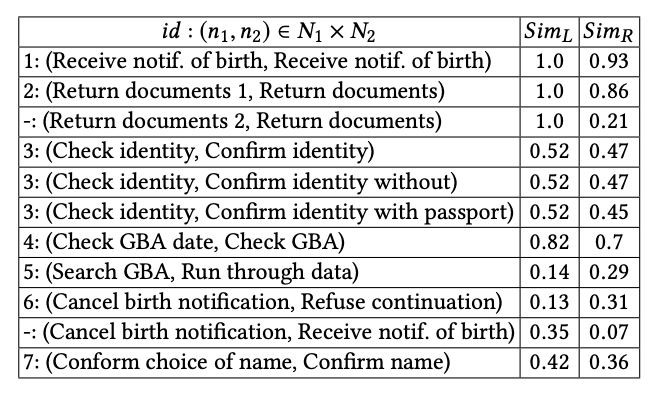
\includegraphics[width = \textwidth]{Figures/Fig_8.PNG}
    \caption{Similarity Score (SimL and SimR) of the application of desired aproach \cite{ref22}}
    \label{fig:8}
\end{figure}

However, the similarity score of (Cancel birth notice, receive birth notification) was reduced from SimL = 0.35 to SimR = 0.07. As a result, the matching algorithm now excludes this activity pair. The similarity score of (Return documents 2, Return documents) was also reduced from SimL = 1.0 to SimR = 0.21. Using a matching method that neglects the process model structure, we can get rid of this activity pair. The similarity scores for matches 1, 2, 3, and 7 declined somewhat. This reduction was caused by some of the activities of their non-similar neighbors. These couples, however, remained the best.\newline

Figure 2 depicts similarity based on labels (SimL) vs Similarity based on our alogrithm (i.e. Similarity Resonance) (SimR) for two university admission processes with their matching techniques. For $\alpha$ = 0.9 and after the first iteration: (Invite for Interview and Invite for aptitude test) = 0.9*(5/19 * Sim0(Assess Applicant, Check if bachelor is sufficient) + 5/19 * Sim0(Check documents, Check if application is complete)+....)+ 0.1* SimL(Invite for Interview and Invite for aptitude test) = 0.1278.
As you can see, the matches' similarity scores improved from SimL =  0.14 to SimR = 0.4 for Receive online application and Receive application form. It also applies to checking documents, checking if the application is complete, Assess the applicant and check if the application is complete. As the similarity scores of the matches went from SimL = 0.12 and SimL = 0.1 to SimR = 0.47 and SimR = 0.41.However, for checking documents, and checking whether the bachelor is sufficient and Invite for interview and invite for aptitude test the similarity scores of the matches decreased from SimL 0.32 to SimR 0.3 and SimL 0.34 to SimR 0.24 respectively, allowing us to exclude this activity pair for improved accuracy.
\begin{figure}
    \centering
    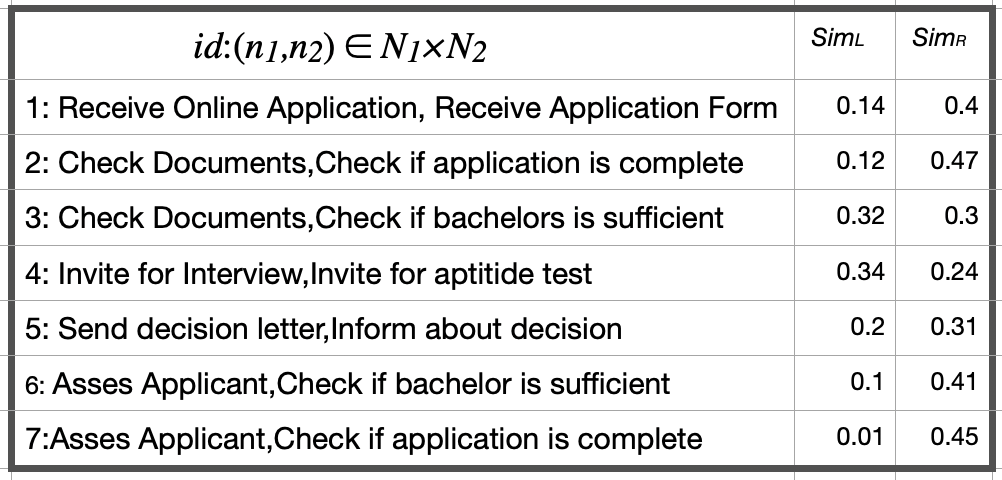
\includegraphics[width = \textwidth]{Figures/Fig_9.PNG}
    \caption{Similarity Score (SimL and SimR) of the application of desired aproach}
    \label{fig:9}
\end{figure}

\section{Conclusion and Future Work}
The paper discusses how to quantify global contextual similarity among activities using a newly developed similarity metric(i.e.Similarity Resonance). According to experimental data, similarity resonance enhances the precision of process matching.The paper's similarity resonance iterative approach is based on Google's Page Rank algorithm for ranking web nodes. The context of an activity is represented by its neighbourhood then, if the neighbourhoods of two activities are comparable, they are considered similar. This leads to iterative approach, in which similarity scores between activities are assigned based on similarity among their neighbours, and the resulting similarity scores are promulgated to neighbouring activities in each stage until convergence. It is important to note that the similarity propagation coefficient is essential to this algorithm. In this study, the paper defines a coefficient based on prior similarity. In the future, we are likely to look at more techniques that take into account other factors, including behavioural and structural relationships between matched activities and their neighbours. Exploring the concept of context is another possibility for future work. Currently, the paper uses precedence relationships to describe the context of an activity. Further, the plan is to investigate how other types of behavioural connections (such as parallelism and choice) affect similarity resonance and matching accuracy.

\bibliographystyle{splncs04}
\begin{thebibliography}{9}
\bibitem{ref1} 
Glen Jeh and Jennifer Widom. 2002. \textit{“SimRank: a measure of structural-context similarity. ”} In Proceedings of the Eighth ACM SIGKDD International Conference on Knowledge Discovery and Data Mining. 538–543.

\bibitem{ref2}
 B. Schellekens \textit{“Marlon Dumas, Wil M. P. van der Aalst, and Arthur H. M. ter Hofstede. 2005”} Master Thesis, Technische Universiteit Eindhoven, 2009.

\bibitem{ref3}
Christopher Klinkmüller, Henrik Leopold, Ingo Weber,Jan Mendling and André Ludwig. 2014. \textit{“ Improving Process Model Matching through User Feedback.”} In Business Process Management - 12th International Conference, BPM. Proceedings. 84–100.

\bibitem{ref4}
 Elena Kuss,Henrik Leopold,Hanvander Aa, Heiner Stuckenschmidt,and Hajo A. Reijers. 2016. \textit{“Probabilistic Evaluation of Process Model Matching Techniques.  ”} In Conceptual Modeling - 35th International Conference, ER. Proceedings. 279–292.

\bibitem{ref5}
Chung-Shou Liao,Kanghao Lu, Michael Baym,Rohit Singh,and Bonnie Berger. 2009. \textit{“IsoRankN: spectral methods for global alignment of multiple protein networks Bioinformatics 25, 12 (2009), i253–i258.”}.

\bibitem{ref6}
W. van der Aalst, M. Schonenberg, and M. Song, \textit{“Time prediction based on process mining,”} Information Systems, vol. 36, no. 2, pp.450–475, Apr. 2011.

\bibitem{ref7}
] Dekang Lin. 1998. \textit{“ An Information-Theoretic Definition of Similarity. In Pro- ceedings of the Fifteenth International Conference on Machine Learning (ICML). 296–304.”}

\bibitem{ref8}
Therani Madhusudan, J. Leon Zhao, and Byron Marshall. 2004.\textit{“A case-based reasoning framework for workflow model management. Data Knowl. Eng. 50, 1 (2004), 87–115.”} 

\bibitem{ref9}
 Sergey Melnik, Hector Garcia-Molina, and Erhard Rahm. 2002. Similarity Flood- ing:\textit{“ A Versatile Graph Matching Algorithm and Its Application to Schema Match- ing.”} In Proceedings of the 18th International Conference on Data Engineering. 117–128.

\bibitem{ref10}
Wil M. P. van der Aalst. 2016.  \textit{“Process Mining - Data Science in Action, Second Edition. Springer.”}

\bibitem{ref11}
W. M. P. van der Aalst, Process Mining - Discovery, Conformance
and Enhancement of Business Processes, 1st ed. Springer, 2011.

\bibitem{ref12}
W. M. P. van der Aalst, V. Rubin, E. Verbeek, B. F. van Dongen,
E. Kindler, and C. W. G¨unther, \textit{“Process mining: a two-step approach to balance between underfitting and overfitting,”} Software \& Systems Modeling, vol. 9, no. 1, pp. 87–111, Nov. 2008.

\bibitem{ref13}
J. Han, M. Pei, and K. Jian, Data Mining Concepts and Techniques,
3rd ed. Elsevier Science Publishers B. V., 2012.

\bibitem{ref14}
C. D. Manning, P. Raghavan, and H. Sch¨utze, Introduction to Information Retrieval, 1st ed. Cambrige University Press, 2008.

\bibitem{ref15}
T. M. Mitchell, Machine Learning, 1st ed. McGraw-Hill, 1997.

\bibitem{ref16}
D. Basak, S. Pal, and D. C. Patranabis, \textit{“Support Vector Regression,”} Neural Information Processing - Letters and Reviews, vol. 10, no. 10,pp. 203–224, 2007.

\bibitem{ref17}
H. Drucker, C. Burges, L. Kaufman, A. Smola, and V. Vapnik, \textit{“Support Vector Regression Machines,”} Neural Information Processing Systems, vol. 1, pp. 155–161, 1996.

\bibitem{ref18}
Wil M. P. van der Aalst, Marcello La Rosa, and Flávia Maria Santoro. 2016. \textit{“Busi- ness Process Management - Don’t Forget to Improve the Process! Business  Information Systems Engineering 58, 1 (2016), 1–6.} 

\bibitem{ref19}
Remco M. Dijkman, Marcello La Rosa, and Hajo A. Reijers. 2012.  \textit{“Managing large collections of business process models - Current techniques and challenges. Computers in Industry 63, 2 (2012), 91–97.”}

\bibitem{ref20}
Marlon Dumas, Wil M. P. van der Aalst, and Arthur H. M. ter Hofstede. 2005. \textit{“Process-Aware Information Systems: Bridging People and Software Through Process
Technology. Wiley.”}

\bibitem{ref21}
J. Shawe-Taylor and N. Cristianini, Kernel methods for pattern analysis.Cambridge University Press, 2004.

\bibitem{ref22}
Minsu Cho, Jungmin Lee, and Kyoung Mu Lee. 2010. \textit{"Reweighted Random Walks for Graph Matching."} In Computer Vision - ECCV - 11th European Conference on Computer Vision. Proceedings, Part V. 492–505.


\bibitem{ref23}
TheICoPFrame- work: Identification of Correspondences between Process Models. In Advanced Information Systems Engineering, 22nd International Conference, CAiSE. Proceed- ings. 483–498.

\bibitem{ref24}
Matthias Weidlich,Tomer Sagi, \textit{"Predicting the Quality of Process Model Matching"}
\bibitem{ref25}
Khurram Shahzad, Ifrah Pervaz, Rao Muhammad Adeel Nawab.\textit{"WordNet-based Semantic Similarity Measures for Process Model Matching"}
\end{thebibliography}
%

\end{document}
